\documentclass[journal, 10pt, twocolumn]{IEEEtran}
\usepackage[utf8]{inputenc}
\usepackage[spanish]{babel}
\usepackage{amsmath,amsfonts,amssymb}
\usepackage{graphicx}
\usepackage{float}
\usepackage{cite}
\usepackage{booktabs}
\usepackage{hyperref}
\usepackage{array}

\title{Caracterización experimental y diseño de un controlador PID para
       un péndulo invertido accionado mediante hélice}

\author{Juan Manuel Beltran Botello - jbeltranbo@unal.edu.co\\
		Nicolas Plata Molano - nplata@unal.edu.co\\
		Oscar Jhonadairo Siabato Leon osiabato@unal.edu.co\\
	    Sergio Andres Bolaños Penagos - sboalnosp@unal.edu.co\\
        Facultad de Ingeniería --- Técnicas de Control}

\begin{document}

\maketitle

% -------------------------------------------------------
\begin{abstract}
Se presenta la identificación experimental, validación en Simulink y diseño
preliminar de un controlador PID para un péndulo invertido accionado por
hélice. Mediante tres tipos de ensayos se obtuvieron los parámetros físicos
de la planta: torque gravitacional, ganancia del actuador, inercia y fricción.
El modelo no lineal implementado en Simulink reprodujo los experimentos de
escalón con un $R^2$ promedio de $0.943$ y un RMSE promedio de $3.37^\circ$.
A partir de la planta linealizada en $\theta_0=70^\circ$ se obtuvo un
controlador PID con $K_p=0.28$, $K_i=1.0$, $K_d=0.20$ y $N=100$.
\end{abstract}

\begin{IEEEkeywords}
Control PID, péndulo invertido, hélice, identificación paramétrica,
oscilación libre, validación experimental, Simulink.
\end{IEEEkeywords}

% ===============================================================
\section{Introducción y montaje experimental}
% ===============================================================

El sistema consiste en una barra articulada cuyo ángulo se regula mediante
el torque producido por una hélice acoplada a un motor DC. Dado que la
dinámica es intrínsecamente no lineal y depende de parámetros físicos del
montaje, antes de diseñar el controlador fue necesario identificar
experimentalmente: el torque gravitacional~$Mgl$, la ganancia entre PWM y
torque~$K_{\tau,\mathrm{PWM}}$, la zona muerta del actuador, el momento de
inercia~$J$ y el coeficiente de fricción viscosa~$b$. El objetivo es
obtener un modelo que reproduzca adecuadamente el comportamiento de la
planta, validarlo en Simulink y utilizarlo para diseñar un controlador PID
alrededor del punto de operación deseado~\cite{ogata,astrom}.

El montaje experimental (Fig.~\ref{fig:montaje}) comprende una estructura
de acrílico que fija el eje de rotación de la barra, un motor DC con hélice
montado en uno de los extremos, un sensor de posición angular, un puente H
L298N como etapa de potencia y una tarjeta Arduino que genera la señal PWM
y adquiere el ángulo. La variable manipulada es el ciclo de trabajo del PWM
(\%) y la variable controlada es el ángulo de la barra (grados).

\begin{figure}[!t]
  \centering
  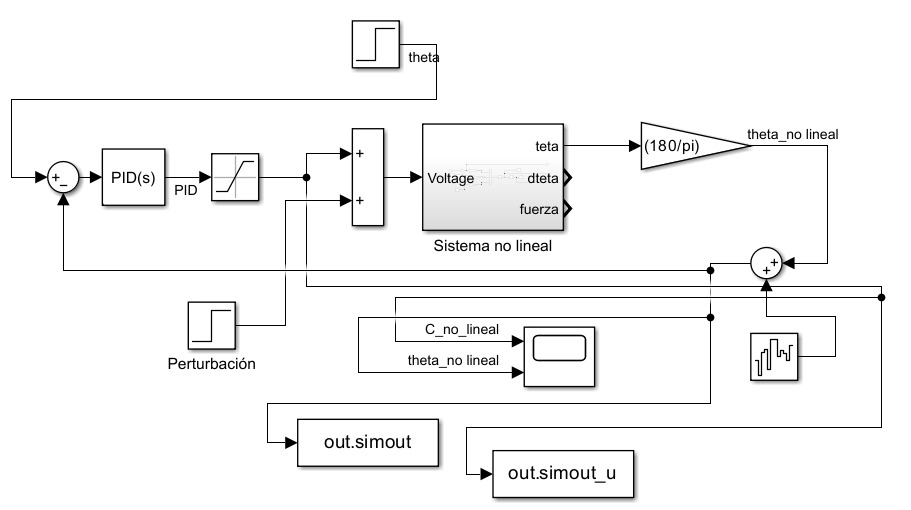
\includegraphics[width=0.85\linewidth]{figuras/Lazo_cerrado.jpeg}
  \caption{Montaje experimental del péndulo accionado mediante hélice
           utilizado para la caracterización de la planta.}
  \label{fig:montaje}
\end{figure}

% ===============================================================
\section{Modelo matemático}
% ===============================================================

Aplicando la segunda ley de Newton para rotación alrededor del eje del
pivote, el balance de torques resulta~\cite{ogata}:

\begin{equation}
  J\,\ddot{\theta} = \tau_h - b\,\dot{\theta} - Mgl\sin(\theta)
  \label{eq:dinamica}
\end{equation}

donde $\tau_h = K_{\tau,\mathrm{PWM}}\cdot u$ es el torque producido por
la hélice, $b\,\dot{\theta}$ representa la disipación viscosa y
$Mgl\sin(\theta)$ es el torque gravitacional. El modelo en variables de
estado con $x_1=\theta$, $x_2=\dot{\theta}$ es:

\begin{equation}
  \dot{x}_1 = x_2, \quad
  \dot{x}_2 = \frac{K_{\tau,\mathrm{PWM}}\,u - b\,x_2
               - Mgl\sin(x_1)}{J}
  \label{eq:estados}
\end{equation}

El modelo asume cuerpo rígido, parámetros constantes y fricción
principalmente viscosa. No incluye fricción de Coulomb, holguras,
retardo del motor ni flexibilidad estructural.

% ===============================================================
\section{Caracterización experimental}
% ===============================================================

\subsection{Caracterización cuasiestática}

Se aplicaron diferentes valores constantes de PWM, se esperó el equilibrio
angular en cada nivel, se repitió en cuatro series y se promediaron los
resultados. En el equilibrio ($\ddot{\theta}=\dot{\theta}=0$), la
Ec.~(\ref{eq:dinamica}) se reduce a $K_{\tau,\mathrm{PWM}}\cdot u_{\mathrm{eq}}
= Mgl\sin(\theta_{\mathrm{eq}})$, de donde se extraen $Mgl$ y
$K_{\tau,\mathrm{PWM}}$ por mínimos cuadrados. El diagnóstico de la zona muerta
se realizó mediante un ajuste afín adicional. Los parámetros obtenidos se
presentan en la Tabla~\ref{tab:parametros}.

\begin{figure}[!t]
  \centering
  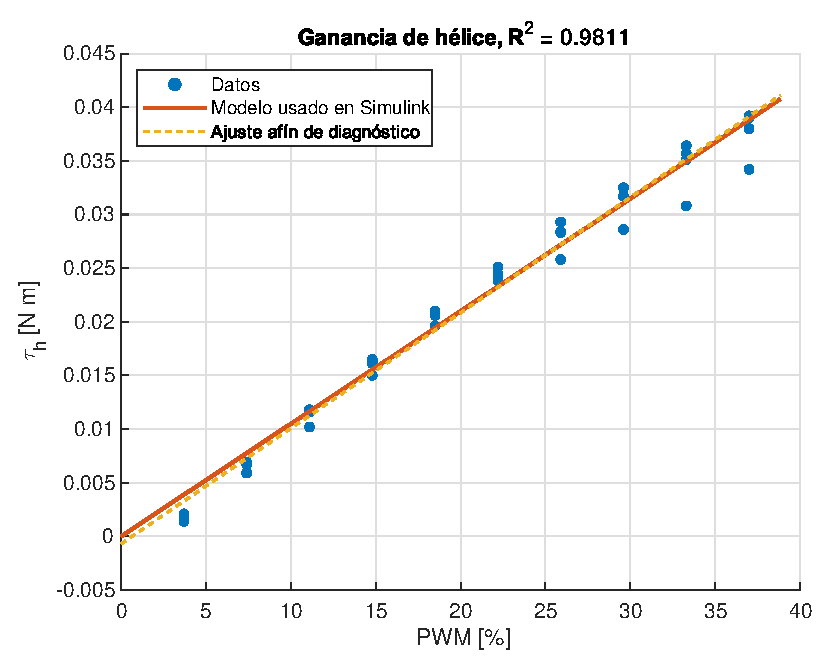
\includegraphics[width=\linewidth]{figuras/Ganancia_estatica.eps}
  \caption{Experimento cuasiestático: relación PWM--torque (izq.) y
           ángulo--torque gravitacional $Mgl\sin(\theta)$ (der.).}
  \label{fig:cuasi}
\end{figure}

El parámetro $Mgl$ determina la magnitud del par gravitacional para cada
ángulo, mientras que $K_{\tau,\mathrm{PWM}}$ cuantifica el incremento de
torque de la hélice por cada punto porcentual de PWM. La dispersión de las
mediciones es moderada, lo que indica que la aproximación lineal es
adecuada dentro del rango de trabajo~\cite{ljung}.

\subsection{Identificación de inercia y fricción}

Se realizaron ensayos de oscilación libre con el motor apagado
($u = 0$). Para cada ensayo se detectaron los máximos de la señal, se
calculó el período amortiguado $T_d$, se ajustó la envolvente exponencial
y se estimaron los parámetros mediante las relaciones:

\begin{align}
  \delta &= \ln\!\left(\frac{A_k}{A_{k+1}}\right),\quad
  \zeta = \frac{\delta}{\sqrt{4\pi^2+\delta^2}}, \notag \\
  \omega_n &= \frac{2\pi}{T_d\sqrt{1-\zeta^2}},\quad
  J = \frac{Mgl\cos\theta_0}{\omega_n^2},\quad
  b = 2\zeta\omega_n J
  \label{eq:libre}
\end{align}

donde $A_k$ son amplitudes de picos consecutivos. Los resultados promediados
sobre los ensayos se muestran en la Tabla~\ref{tab:parametros}.

\begin{figure}[!t]
  \centering
  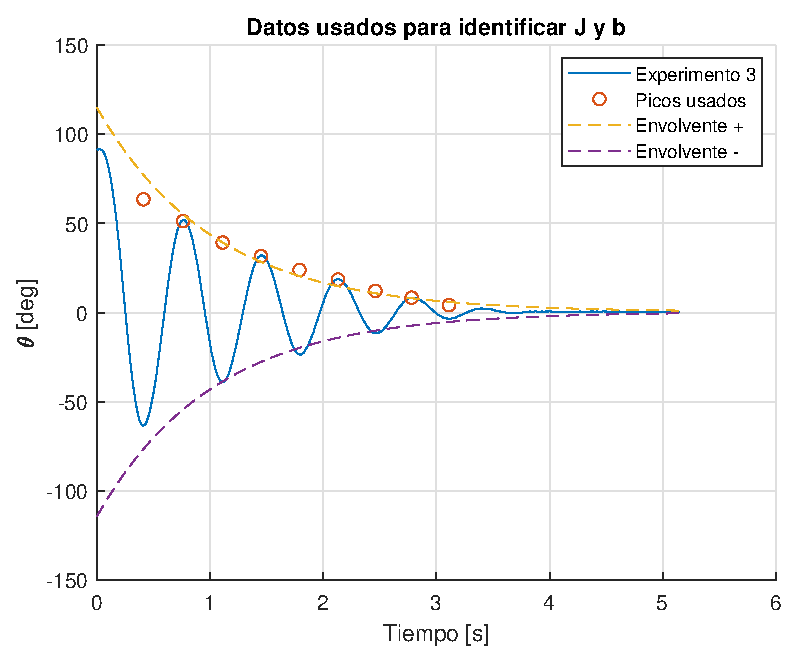
\includegraphics[width=\linewidth]{figuras/Oscilacion_libre.eps}
  \caption{Ensayo representativo de oscilación libre: decaimiento
           exponencial del ángulo a partir del cual se estiman $J$ y $b$.}
  \label{fig:libre}
\end{figure}

El $R^2$ promedio de $0.959$ del ajuste de la envolvente indica que el
decaimiento exponencial representa razonablemente la tendencia de las
oscilaciones, aunque no captura todos los fenómenos de fricción
presentes en el sistema real~\cite{ljung}.

\begin{table}[H]
  \centering
  \caption{Parámetros identificados experimentalmente.}
  \label{tab:parametros}
  \begin{tabular}{lcc}
    \toprule
    Parámetro & Valor & Unidad \\
    \midrule
    $Mgl$                          & $3.9244\times10^{-2}$  & N$\cdot$m \\
    $K_{\tau,\mathrm{PWM}}$        & $1.0492\times10^{-3}$  & N$\cdot$m/\%PWM \\
    $K_{\tau,V}$                   & $1.1658\times10^{-2}$  & N$\cdot$m/V \\
    Zona muerta                    & $0.649$                & \%PWM \\
    $J$                            & $4.2860\times10^{-4}$  & kg$\cdot$m$^2$ \\
    $b$                            & $8.3032\times10^{-4}$  & N$\cdot$m$\cdot$s/rad \\
    $T_d$ (promedio)               & $0.662$                & s \\
    $R^2$ envolvente (promedio)    & $0.959$                & --- \\
    \bottomrule
  \end{tabular}
\end{table}

% ===============================================================
\section{Implementación y validación en Simulink}
% ===============================================================

La integración numérica de la Ec.~(\ref{eq:dinamica}) se realizó
íntegramente en el modelo \texttt{modelo\_proyecto.slx}. MATLAB actúa
como orquestador: lee los datos de \texttt{Experimentos.xlsx}, construye
la señal \texttt{entradaPWM}, asigna los parámetros y condiciones iniciales,
ejecuta Simulink, recupera \texttt{simout} e interpola las señales para
calcular las métricas de error~\cite{fromws}. Los bloques principales del
modelo son: \textit{From Workspace} (señal de entrada), subsistema de la
planta (torque de hélice, gravedad y fricción), dos integradores (velocidad
y posición) y \textit{To Workspace} (salida en grados).

\subsection{Validación con oscilaciones libres}

Con $u=0$ y las condiciones iniciales medidas, el modelo reproduce la
frecuencia de oscilación y la tendencia general del decaimiento, pero
subestima la disipación real. Las diferencias se atribuyen a fricción
de Coulomb, fricción estática, torque generado por los cables, holguras y
cuantización del sensor. Los resultados promedio se presentan en la
Tabla~\ref{tab:metricas}.

\subsection{Validación con experimentos de escalón}

Los tres ensayos de escalón independientes enviaron la señal PWM experimental
completa al modelo de Simulink y compararon la salida angular simulada con la
medida. Los resultados individuales y promedio se incluyen en la
Tabla~\ref{tab:metricas}.

\begin{figure}[!t]
  \centering
  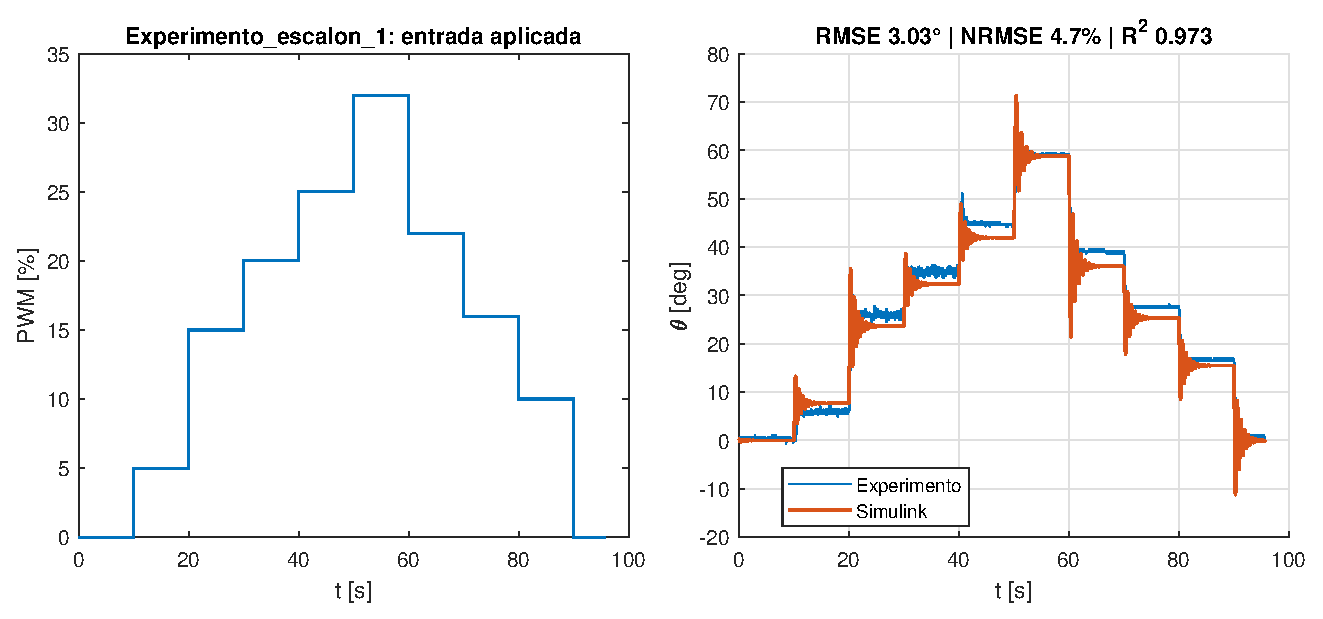
\includegraphics[width=\linewidth]{figuras/Experimento_escalones_1.eps}\\[2pt]
  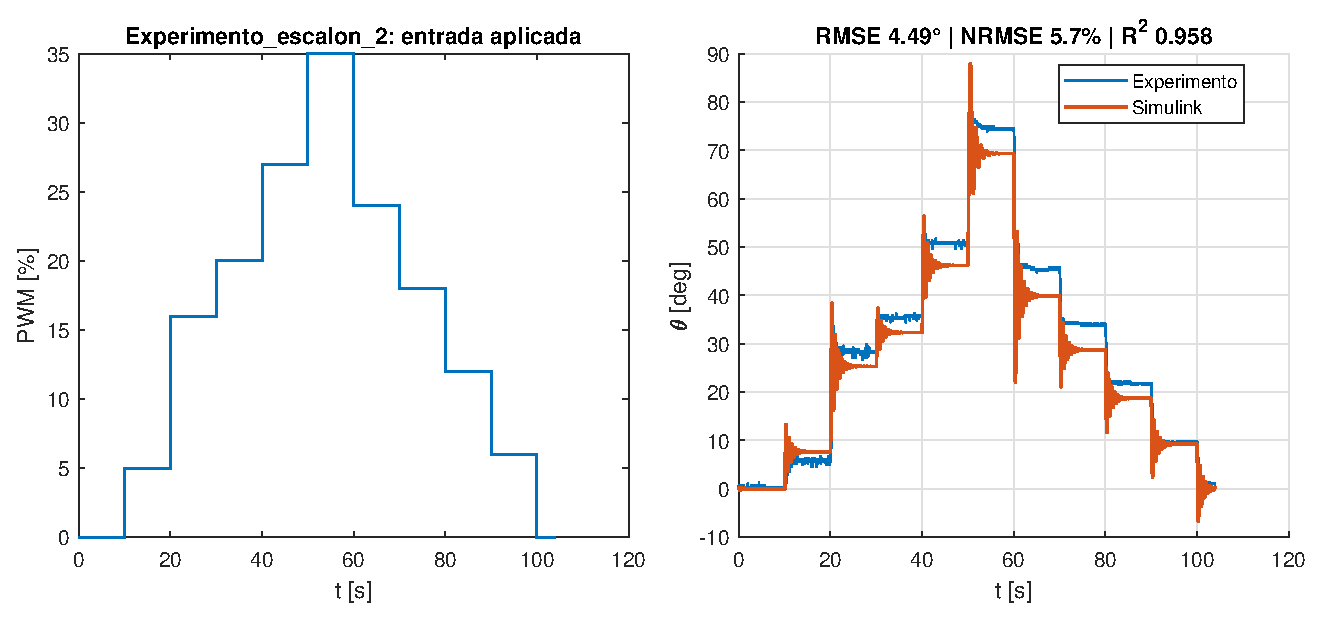
\includegraphics[width=\linewidth]{figuras/Experimento_escalones_2.eps}\\[2pt]
  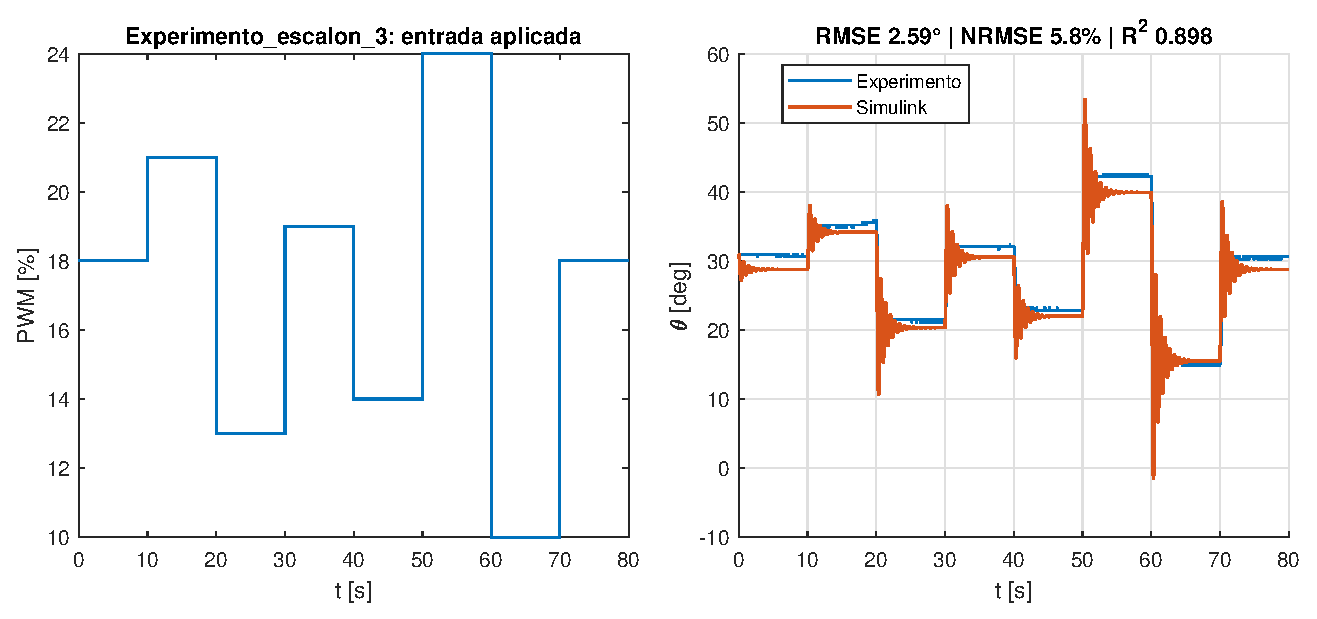
\includegraphics[width=\linewidth]{figuras/Experimento_escalones_3.eps}
  \caption{Validación con escalones: PWM aplicado (izq.) y ángulo
           medido vs.~simulado (der.) para los tres ensayos.}
  \label{fig:escalones}
\end{figure}

\begin{table}[H]
  \centering
  \caption{Métricas de validación del modelo en Simulink.}
  \label{tab:metricas}
  \begin{tabular}{lcccc}
    \toprule
    Experimento & RMSE ($^\circ$) & NRMSE (\%) & $R^2$ \\
    \midrule
    Oscilación libre (prom.) & 9.16 & 5.89 & 0.852 \\
    \midrule
    Escalón 1  & 3.03 & 4.70 & 0.973 \\
    Escalón 2  & 4.49 & 5.74 & 0.958 \\
    Escalón 3  & 2.59 & 5.79 & 0.898 \\
    Escalones (prom.) & \textbf{3.37} & \textbf{5.41} & \textbf{0.943} \\
    \bottomrule
  \end{tabular}
\end{table}

El ajuste es notablemente mejor en los escalones que en las oscilaciones
libres porque durante los escalones domina el torque de la hélice, que el
modelo captura con buena precisión. En las oscilaciones libres el peso de
los fenómenos de fricción no lineal es mayor. Un $R^2$ promedio de $0.943$
y un NRMSE promedio de $5.41\,\text{\%}$ en los escalones confirman que la dinámica
forzada fue identificada adecuadamente y que el modelo es apropiado para el
diseño preliminar del controlador~\cite{ljung}.

% ===============================================================
\section{Linealización y diseño del PID}
% ===============================================================

\subsection{Planta linealizada}

El sistema se linealizó alrededor de $\theta_0 = 70^\circ$. Imponiendo
$\dot{\theta}=0$ y $\ddot{\theta}=0$ se determina la entrada de equilibrio
$u_0$ tal que el torque de la hélice compensa exactamente el torque
gravitacional. Introduciendo perturbaciones pequeñas
$\theta = \theta_0+\Delta\theta$, $u = u_0+\Delta u$ y expandiendo
$\sin(\theta)$ en serie de Taylor de primer orden, se obtiene la planta
linealizada~\cite{ogata,astrom}:

\begin{equation}
  G(s) = \frac{140.3}{s^2 + 1.937\,s + 31.32}
  \label{eq:Gs}
\end{equation}

con $\Delta u$ en \%PWM y $\Delta\theta$ en grados. Los polos complejos
conjugados con parte real negativa confirman que el sistema linealizado
es estable en lazo abierto en este punto. La frecuencia natural es
$\omega_n \approx 5.60$\,rad/s con $\zeta \approx 0.17$. Este modelo es
local y solo representa movimientos pequeños alrededor de $70^\circ$.

\begin{figure}[!t]
  \centering
  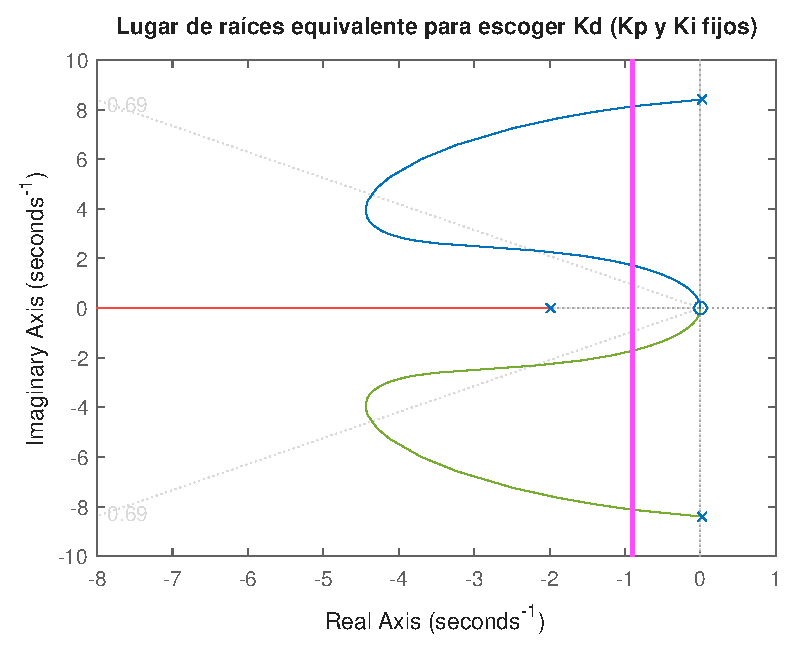
\includegraphics[width=\linewidth]{figuras/RootLocus_PI.eps}
  \caption{Lugar de las raíces del sistema en lazo cerrado empleado
           para la sintonización del controlador PID.}
  \label{fig:rlocus}
\end{figure}

\subsection{Controlador PID}

Se seleccionó un controlador PID con filtro derivativo~\cite{pidsimulink}:

\begin{equation}
  C(s) = K_p + \frac{K_i}{s} + \frac{K_d\,N\,s}{s+N}
       = \frac{20.28\,s^2 + 29\,s + 100}{s^2 + 100\,s}
  \label{eq:Cs}
\end{equation}

Los parámetros se presentan en la Tabla~\ref{tab:pid}. $K_p$ aumenta la
rapidez y reduce el error; $K_i$ elimina el error estacionario; $K_d$
incrementa el amortiguamiento efectivo; y $N = 100$ limita la
amplificación de ruido en el término derivativo sin distorsionar la acción
de control en el rango de frecuencias de interés~\cite{pidsimulink}.

\begin{table}[H]
  \centering
  \caption{Parámetros del controlador PID diseñado.}
  \label{tab:pid}
  \begin{tabular}{lcl}
    \toprule
    Parámetro & Valor & Descripción \\
    \midrule
    $K_p$ & $0.28$  & Ganancia proporcional \\
    $K_i$ & $1.0$   & Ganancia integral \\
    $K_d$ & $0.20$  & Ganancia derivativa \\
    $N$   & $100$   & Constante del filtro derivativo \\
    \bottomrule
  \end{tabular}
\end{table}

Estas ganancias corresponden a un diseño inicial basado en el modelo
linealizado. La validación posterior debe verificar el desempeño en
el modelo no lineal considerando: saturación del PWM, zona muerta,
Anti-Windup, ruido y perturbaciones.

\begin{figure}[!t]
  \centering
  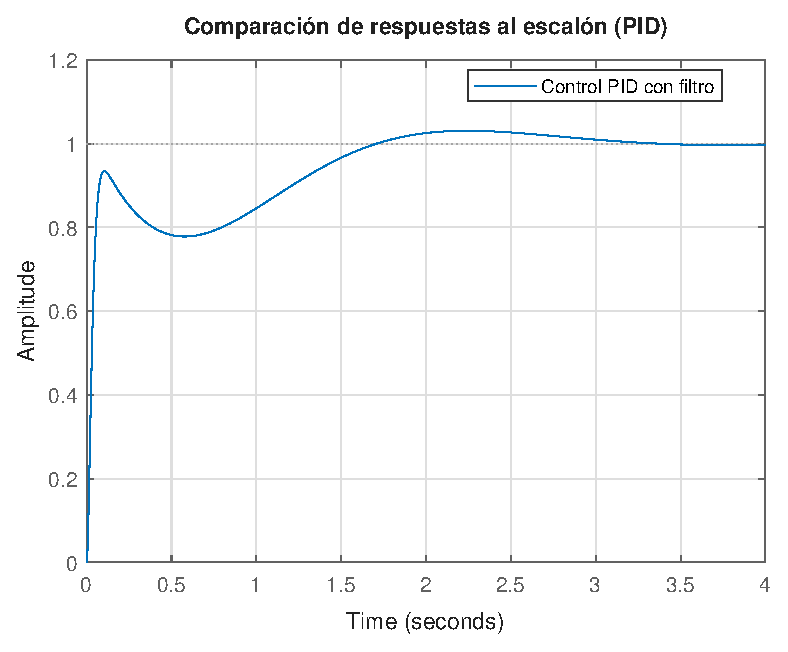
\includegraphics[width=\linewidth]{figuras/Step_PID.eps}
  \caption{Respuesta al paso del sistema con controlador PID en lazo
           cerrado (simulación en modelo no lineal).}
  \label{fig:step_pid}
\end{figure}

\begin{figure}[!t]
  \centering
  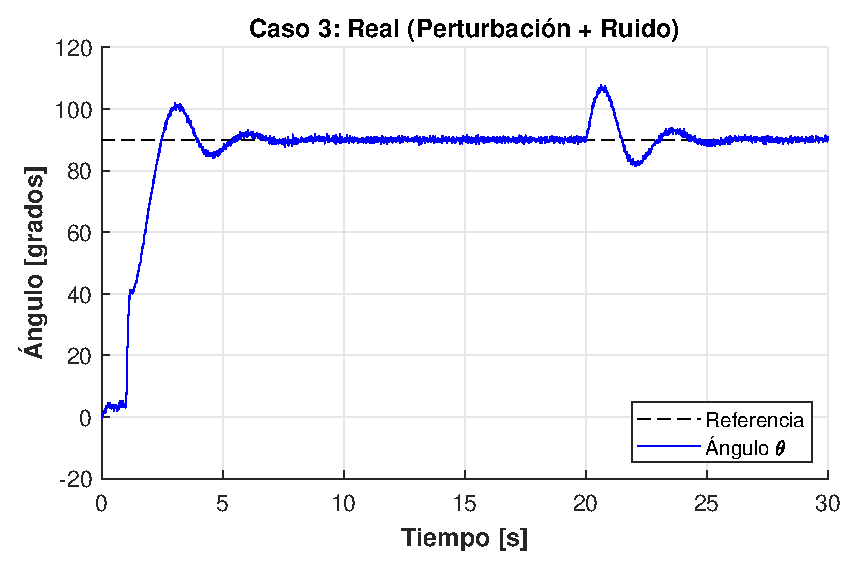
\includegraphics[width=\linewidth]{figuras/Respuesta_90_Caso_3.eps}
  \caption{Caso 3 -- Ruido: respuesta angular del péndulo con ruido
           de medición activo. El controlador mantiene la posición
           estable en torno a la referencia.}
  \label{fig:caso3}
\end{figure}

% ===============================================================
\section{Discusión y conclusiones}
% ===============================================================

La caracterización cuasiestática permitió estimar la ganancia del actuador,
el torque gravitacional y la zona muerta con una dispersión moderada,
compatible con la hipótesis de linealidad en el rango de trabajo. Los
ensayos de oscilación libre entregaron estimaciones de $J$ y $b$ con un
$R^2$ de envolvente promedio de $0.959$, indicando que el decaimiento
exponencial es una aproximación razonable aunque no captura la fricción no
lineal completa ($R^2$ de validación en lazo abierto de $0.852$).

Los experimentos de escalón confirman que la ganancia del actuador y la
dinámica dominante fueron identificadas adecuadamente ($R^2 = 0.943$,
RMSE $= 3.37^\circ$). La diferencia de ajuste entre oscilaciones libres y
escalones sugiere que la fricción real incluye componentes de Coulomb y
estática que el modelo viscoso no representa por completo.

El modelo identificado es apropiado para el diseño preliminar del
controlador, pero puede mejorarse incorporando: fricción de Coulomb, zona
muerta y saturación explícitas, y una dinámica de primer orden para el
conjunto motor--hélice. El controlador PID diseñado debe validarse en el
modelo no lineal e implementarse con estrategia Anti-Windup antes de su
uso en el sistema físico.

% -------------------------------------------------------
\bibliographystyle{IEEEtran}
\begin{thebibliography}{5}

\bibitem{ogata}
K.~Ogata,
\textit{Modern Control Engineering}, 5th~ed.
Pearson, 2010.

\bibitem{astrom}
K.~J.~Åström and R.~M.~Murray,
\textit{Feedback Systems: An Introduction for Scientists and Engineers}.
Princeton University Press, 2008.

\bibitem{ljung}
L.~Ljung,
\textit{System Identification: Theory for the User}, 2nd~ed.
Prentice Hall, 1999.

\bibitem{fromws}
MathWorks, ``From Workspace,''
\textit{Simulink Documentation}, 2024.
[Online]. Available: \url{https://www.mathworks.com/help/simulink}

\bibitem{pidsimulink}
MathWorks, ``PID Controller,''
\textit{Simulink Documentation}, 2024.
[Online]. Available: \url{https://www.mathworks.com/help/simulink}

\end{thebibliography}

\end{document}
